\chapter{Gra karciana Love Letter}
\label{cha:rozdz2}

W tym rozdziale opisuję kontekst oraz zasady gry Love Letter. Tłumaczę działanie każdej karty oraz przedstawiam główny cel gry - wygranie określonej ilości rund. Następnie formułuję zagadnienie w sposób matematyczny. Wszystkie załączone zdjęcia oraz instrukcja zaczerpnięte są z [\ref{bib:loveLetterGame}] oraz [\ref{bib:loveLetterWebsite}].

\begin{figure}[h]
	\centering
	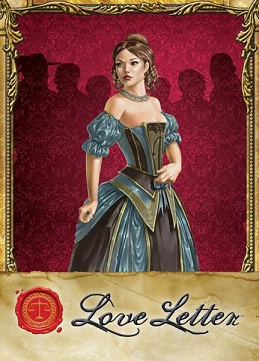
\includegraphics{Resources/ll_main_image.png}
	\caption{Love Letter - okładka} 
	\label{fig:llMainImage}
\end{figure}

\section{Opis zasad gry}
\label{sec:opisGry}
W trakcie gry wcielamy się w rolę jednego z adoratorów księżniczki starającego się o zdobycie jej serca. W tym celu przygotowaliśmy list miłosny, który chcemy jej dostarczyć. Niestety, księżniczka pogrążona jest obecnie w żałobie i nie przyjmuje do siebie nikogo obcego, w związku z czym musimy znaleźć inny sposób na przekazanie jej naszego listu. Oprócz księżniczki, na dworze znajdują się inne postacie, z których każda ma mniejszy lub większy dostęp do komnat naszej wybranki i może oddać jej list. Przekazujemy więc naszą przesyłkę swojemu tajnemu posłańcowi, a na koniec gry księżniczka jako pierwszy przeczyta ten list, który został przekazany przez najbardziej zaufaną postać. Serce wybranki zdobywa gracz, który jako pierwszy przekaże w ten sposób od 4 do 7 listów, w zależności od liczby graczy.

\section*{Cel i ustawienie początkowe}
\label{sec:celIUstawieniePoczatkowe}
Love Letter rozgrywa się jako serię rund. Grę wygrywa gracz o następującej ilości wygranych rund:
\begin{itemize}
	\item 7 w grze na 2 graczy,
	\item 5 w grze na 3 graczy,
	\item 4 w grze na 4 graczy.
\end{itemize}

Ustawienie początkowe każdej rundy wygląda następująco:
\begin{itemize}
	\item przetasuj karty
	\item odrzuć 1 wierzchnią kartę nie odkrywając jej (nie bierze udziału w rundzie),
	\item jeśli gra tylko 2 graczy, odrzuć 3 wierzchnie karty, odkryte,
	\item rozdaj po 1 karcie wszystkim graczom,
	\item jeśli jest to pierwsza runda, grę zaczyna gracz, który jako ostatni był na randce, w przeciwnym wypadku zwycięzca poprzedniej rundy.
\end{itemize}

\section*{Tura gracza i opis kart}
\label{sec:turaGracza}
Podczas swojej tury gracz dociąga jedna kartę ze stosu. Następnie wybiera jedną z dwóch kart, które posiada już na ręce, kładzie ją przed sobą tak, by była widoczna dla wszystkich i zastosowuje opisany na niej efekt - nawet jeśli jest negatywny. Zagrana karta pozostaje odkryta przez całą rundę, a druga pozostaje na ręce. Następnie tura przechodzi na osobę po lewej stronie aktywnego gracza.

W grze znajduje się 16 kart, w 8 typach. Są to kolejno: 4 karty Strażniczki, po 2 karty Kapłana, Barona, Pokojówki i Księcia, oraz po jednej karcie Króla, Hrabiny i Księżniczki. Ich szczegółowy opis wraz z wyglądem znajduje się poniżej:

\clearpage
\begin{figure}[h]
	\centering
	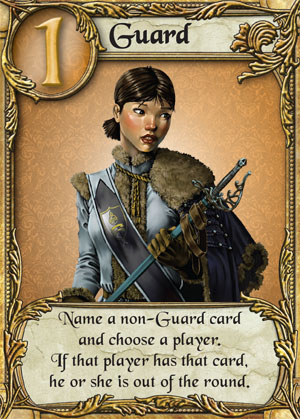
\includegraphics[scale=0.5]{Resources/Love_Letter_Card_Guard.png}
	\caption{Strażniczka} \label{fig:Love_Letter_Card_Guard}
\end{figure}
Na rysunku \ref{fig:Love_Letter_Card_Guard} przedstawiona jest karta typu Strażniczka. Zagrywając tę kartę należy wskazać jednego z pozostałych graczy i odgadnąć kartę którą posiada. Jeśli karta została prawidłowo odgadnięta, wskazany gracz odrzuca ją i przegrywa rundę.

\begin{figure}[h]
	\centering
	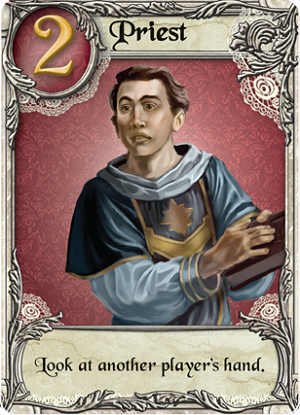
\includegraphics[scale=0.5]{Resources/Love_Letter_Card_Priest.png}
	\caption{Kapłan} \label{fig:Love_Letter_Card_Priest}
\end{figure}
Rysunek \ref{fig:Love_Letter_Card_Priest} przedstawia kartę typu Kapłan. Zagrywając tę kartę należy podglądnąć kartę wybranego gracza.

\clearpage
\begin{figure}[h]
	\centering
	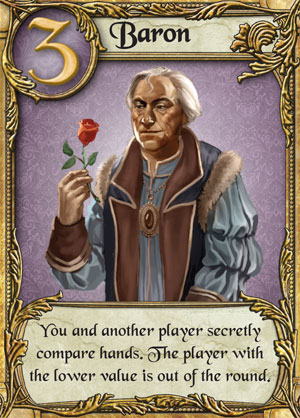
\includegraphics[scale=0.5]{Resources/Love_Letter_Card_Baron.png}
	\caption{Baron - 2 karty} \label{fig:Love_Letter_Card_Baron}
\end{figure}
Na rysunku \ref{fig:Love_Letter_Card_Baron} przedstawiona jest karta typu Baron. Po zagraniu tej karty należy w ukryciu porównać drugą posiadaną kartą z wybranym graczem. Następnie ten gracz, który ma kartę o mniejszej wartości odrzuca swoją kartę i przegrywa rundę. W przypadku remisu nic się nie dzieje.

\begin{figure}[h]
	\centering
	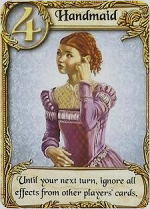
\includegraphics{Resources/Love_Letter_Card_Handmaid.png}
	\caption{Pokojówka - 2 karty} \label{fig:Love_Letter_Card_Handmaid}
\end{figure}
Rysunek \ref{fig:Love_Letter_Card_Handmaid} przedstawia kartę typu Pokojówka. Zagranie tej karty sprawia, że gracz jest niewrażliwy na efekt pozostałych kart do czasu swojej następnej tury.

\clearpage
\begin{figure}[h]
	\centering
	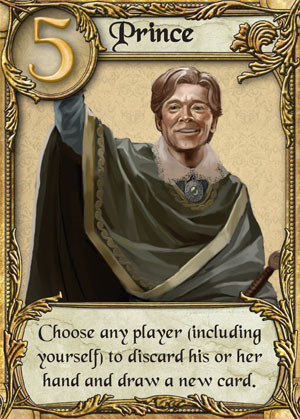
\includegraphics[scale=0.5]{Resources/Love_Letter_Card_Prince.png}
	\caption{Książe - 2 karty} \label{fig:Love_Letter_Card_Prince}
\end{figure}
Na rysunku \ref{fig:Love_Letter_Card_Prince} przedstawiona jest karta typu Książę. Zagranie pozwala wybrać dowolnego gracza (w tym siebie), zmusić go do odrzucenia posiadanej karty i pociągnięcia następnej.

\begin{figure}[h]
	\centering
	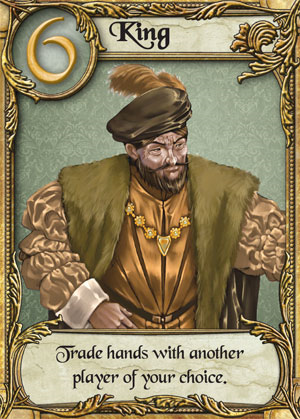
\includegraphics[scale=0.5]{Resources/Love_Letter_Card_King.png}
	\caption{Król - 1 karta} \label{fig:Love_Letter_Card_King}
\end{figure}
Rysunek \ref{fig:Love_Letter_Card_King} przedstawia kartę typu Król. Po jej zagraniu należy wymienić się pozostałą kartą z innym graczem.

\clearpage
\begin{figure}[h]
	\centering
	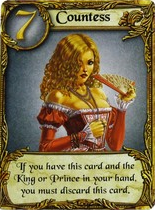
\includegraphics{Resources/Love_Letter_Card_Countess.png}
	\caption{Hrabina - 1 karta} \label{fig:Love_Letter_Card_Countess}
\end{figure}
Rysunek \ref{fig:Love_Letter_Card_Countess} przedstawia kartę typu Hrabina. Ta karta ma działanie pasywne. Nie wywiera efektu po zagraniu, natomiast zmusza gracza do jej zagrania jeśli równocześnie posiada na ręce kartę typu Książę lub Król.

\begin{figure}[h]
	\centering
	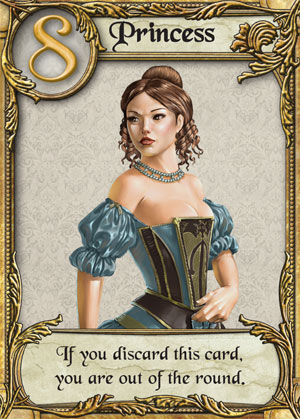
\includegraphics[scale=0.5]{Resources/Love_Letter_Card_Princess.png}
	\caption{Księżniczka - 1 karta} \label{fig:Love_Letter_Card_Princess}
\end{figure}
Na rysunku \ref{fig:Love_Letter_Card_Princess} przedstawiona jest karta typu Księżniczka. Zagranie tej karty oznacza natychmiastową przegraną w rundzie. Ta zasada działa również, gdy gracz został zmuszony do zagrania tej karty, np. przez efekt karty Książe.
\clearpage


\section{Analiza złożoności problemu}
\label{sec:opisProblemu}
Z wyżej przedstawionych zasad wynika, że gra cechuje się wysokim stopniem losowości i jest niedeterministyczna. W związku z tym powstaje pytanie, czy istnieje strategia mieszana$^{[\ref{bib:wiki_StrategiaTeoriaGier}]}$ optymalizująca podejmowane decyzje w taki sposób, by zwiększać szansę wygrania gry. Dla uproszczenia założyłem, że gra będzie rozgrywana przez dwóch graczy.

By móc opracować najlepszą strategię, musiałbym znać wszystkie możliwe scenariusze gry, na podstawie których można by ustalić statystycznie który ruch w danym momencie jest najbardziej opłacalny. Jako scenariusz należy rozumieć wszystkie podjęte przez graczy ruchy w danej rundzie. Wpływ na to mają dwa czynniki:
\begin{itemize}
	\item Kolejność kart w talii na początku rundy
	\item Sposób zagrania karty
\end{itemize}
Dokonałem więc oszacowania, ile takich scenariuszy istnieje. 

W każdej rundzie bierze udział wszystkie 16 kart. Zakładając, że każda z nich jest unikalna, to  liczba wszystkich możliwych kolejności kart to permutacja, którą obliczam wzorem podanym w [\ref{bib:tabliceMatematyczne}]:

\begin{center}
	$P_n = n!$ , gdzie $n\in N^+$
\end{center}

Dla  $n$ = 16, $n!=20 922 789 888 000$. Część kart się powtarza, więc tę liczbę należy jeszcze podzielić przez permutacje powtarzających się kart Strażniczki, Kapłana, Barona, Pokojówki oraz Księcia. Razem jest to $4! * 2! * 2! * 2! * 2! =  384$. Ostatecznie wynika, że liczba unikalnych kolejności kart wynosi: 

\begin{center}
	$20 922 789 888 000 / 32 = 54486432000$ - 54mld, 864mln i 432 tys.
\end{center}

Nie jest to jednak liczba wszystkich dostępnych scenariuszy. Ponieważ w każdej turze gracz zagrywa jedną z dwóch dostępnych kart, a ponadto w przypadku części z nich może podjąć różne decyzje, to kolejność w której gracze dociągną karty z dostępnej talii będzie się wielokrotnie zmieniać w trakcie rozgrywki. Dobrym przykładem jest Książę, który zmusza przeciwnika do odrzucenia posiadanej karty i pociągnięcia następnej. 

By wyznaczyć w liczbę scenariuszy na zadanej kolejności kart, posłużyłem się następującym przybliżeniem:
\begin{itemize}
	\item zgodnie z zasadami gry dla dwóch graczy, odrzucam łącznie 4 pierwsze karty (1 zakryta, 3 odkryte).
	\item rozdaję po 1 karcie obu graczom. Pozostaje 10 kart w talii.
	\item zakładając, że żadna decyzja nie spowoduje przerwania rundy, gracze łącznie 10 razy pociągną kartę, więc podejmą 10 decyzji.
	\item w uproszczeniu, każdą decyzję można przedstawić jako 0 (zagranie posiadanej karty) lub 1 (zagranie pociągniętej karty).
\end{itemize}
Na podstawie powyższego można oszacować, że możliwych scenariuszy dla danej kolejności kart jest $2^{10}=1024$. Łącząc tę liczbę z ilością możliwych kolejności kart, utrzymujemy przybliżoną liczbę scenariuszy:

\begin{center}
	$54486432000 * 1024 = 55794106368000 \approx  5.8*10^{12}$
\end{center}

Z uwagi na rząd wielkości stworzenie strategii na podstawie analizy statystycznej wszystkich dostępnych scenariuszy jest problemem \textit{NP-trudnym}. Z tego powodu, zamiast odpowiadać na pytanie "Jaka jest najlepsza strategia podejmowania decyzji?", dużo łatwiej będzie odpowiedzieć na pytanie "Która z podanych strategii jest najlepsza?", gdyż jest to charakterystyczna cecha problemów klasy \textit{NP}. Kierując się tą zasadą, w następnym rozdziale opisałem wybrane strategie, których skuteczność sprawdzę implementując je w napisanej przeze mnie aplikacji.